\documentclass[12pt,a4paper]{article}
\usepackage{amsfonts, amssymb, amsmath}
\usepackage{fullpage}
\usepackage{parskip} % skip a line instead of indenting
\usepackage{graphicx} % for inserting images
\usepackage{amsthm}
\usepackage{xcolor}
\usepackage{tikz} % for plot

\newtheorem*{rem}{Remark}

\title{Algorithms}
\author{R4 Cheng}
\date{\today}

\newcommand{\Remark}[1]{
  \begin{rem}
    \color{cyan}
    #1
  \end{rem}
}

\begin{document}
\maketitle

\textbf{Def.} Introduction of precise, umambiguous, and correct procedures for solving general problems

We care how many clicks in debug mode

Runtime is expressed by counting the number of steps, as funtion of \textbf{the size of the input}

Asymptotic Notations:

\begin{itemize}
  \item Big $O$: upper bound on the growth rate
  \item Little $o$: "strict" upper bound on the growth rate
  \item Big $\Omega$: lower bound on the growth rate
  \item $\Theta$: tight bound on the growth rate
\end{itemize}

$f(n)$: the runtime of an algorithm for input size $n$

$g(n)$: a simplified function without constants, lower order terms, e.g. $n^2$, $n \log n$

\textbf{Big-O Definition}: It is said $f(n) = O(g(n)) \iff$ there exists a constant $c > 0$ and $n_0 > 0$ such that
$$f(n) \leq c \cdot g(n) \text{ for all } n \geq n_0$$

\textbf{Little-o Definition}:
$$f(n) = o(g(n)) \iff \lim_{n \to \infty} \frac{f(n)}{g(n)} = 0$$

\textbf{Big-$\Omega$ Definition}: It is said $f(n) = \Omega(g(n)) \iff$ there exists a constant $c > 0$ and $n_0 > 0$ such that
$$f(n) \geq c \cdot g(n) \text{ for all } n \geq n_0$$

\subsubsection*{Caveats about constants}

For $\log_4(n)$, is 4 ignorable? No, it matters

\Remark{$log_a(x) = log_a blog_b(x)$}

\includegraphics[width=\textwidth]{./images/common_efficiency_class.png}

\subsection*{Merge Sort}

\[T(n) = 2T(\frac{n}{2}) + 2n + c\]

\Remark{$2n$: compare and copy n elements $= 2n$}

\textbf{Proof}

\[T(n) = 2T(\frac{n}{2}) + 2n + c\]
\[\Rightarrow T(\frac{n}{2}) = 2T(\frac{n}{4}) + (n + c)\]
\[\Rightarrow T(\frac{n}{4}) = 2T(\frac{n}{8}) + (\frac{n}{2} + c)\] Bring in $T(\frac{n}{2})$
\[\Rightarrow T(n) = 2\{2T(\frac{n}{4}) + (n + c)\} + 2n + c\]
\[= 2^2T(\frac{n}{2^2}) + 2 \cdot 2n + c + 2c\] Bring in $T(\frac{n}{4})$
\[= 2^2\{2T(\frac{n}{8}) + (\frac{n}{2} + c)\} + 2 \cdot 2n + c + 2c\]
\[= 2^3T(\frac{n}{2^3}) + 3 \cdot 2n + c + 2c + 4c\]
\[\Rightarrow T(n)= 2^kT(\frac{n}{2^k}) + k \cdot 2n + (2^k-1)c\]

Since $T(1) = 1$, $\frac{n}{2^k} = 1 \Rightarrow k = \log_2(n)$

\[\Rightarrow T(n) = n \cdot 1 + \log_2(n) \cdot 2n + (n-1)c\]
\[\Rightarrow T(n) = O(nlogn) \]

\section*{Master Theorem}

\[T(n) = aT(\frac{n}{b}) + cn^d\]
\[\Rightarrow T(n) = (1 + \frac{a}{b^d}^2 + \cdots + \frac{a}{b^d}^k)cn^d\]

$a$: number of subproblems

$b$: factor by which the problem size is reduced

$d$: exponent in the running time of the "combine" step

\textbf{Case 1}: $a < b^d$, or equiv. $d > log_ba, T(n) = O(n^d)$
$\Rightarrow$ the cost of the "combine" step dominates the cost of the "split" step

\textbf{Case 2}: $a = b^d$, or equiv. $d = log_ba, T(n) = O(n^d \log n)$

\textbf{Case 3}: $a > b^d$, or equiv. $d < log_ba, T(n) = O(n^{log_ba})$

\section*{Smart Selection of Pivot}

Break array $A$ into chunks of fives and find the median of each chunk,
constructing a new array $M$ of medians.

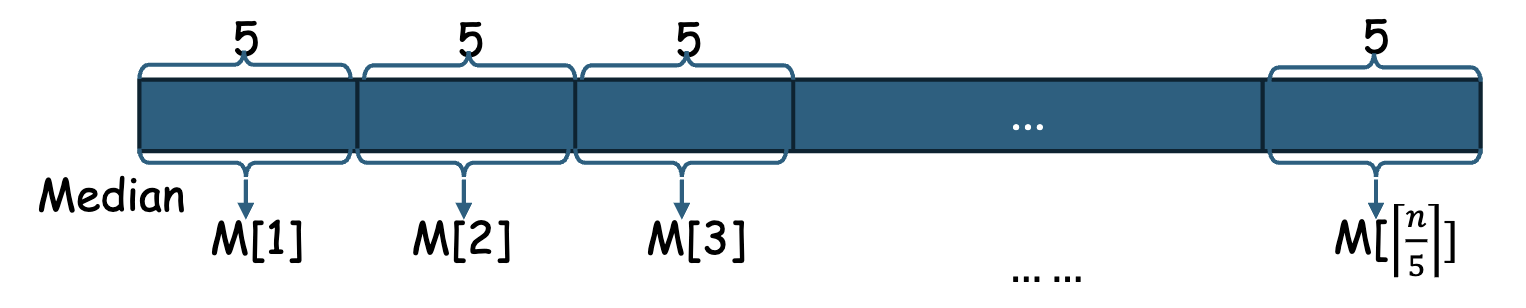
\includegraphics[width=\textwidth]{./images/chunks_of_fives.png}

And \textbf{median} of $M$ aka. $MM$ is the pivot.

\textbf{Claim:} $MM$ is at least $\geq \frac{3}{10}A$ and $\leq \frac{3}{10}A$

\textbf{Proof:} $MM$ is the median of medians, so $\frac{1}{2}$ medians in $M$ are $\leq MM$.
$\because M = \frac{A}{5} \Rightarrow \frac{A}{10}$ medians are $\leq MM$. Moreover, 
For each $M[i]$, there are 3 elements $\leq M[i]$ $\therefore \frac{3A}{10} \leq MM$

\begin{verbatim}
Select(A, k)
1. for i = 1, ..., n/5
2.     M[i] = median (a[5(i-1)+1], 5i)
3. MM = Select(M, n/10)
4. v = index of MM in A
5. r = partition(A, v)
6. if k=r: return A[r]
7. if k<r: Select(A[1,...,r-1], k)
8. if k>r: Select(A[r+1,...,n], k-r)
\end{verbatim}

\[T(n) \leq O(n) + T(n/5) + T(7n/10) \Rightarrow T(n) = O(n)\]

\section*{Dynamic Programming}

\subsection*{Fibonacci}

\[T(n) = T(n-1) + T(n-2) + c\]
\[\Rightarrow T(n) \leq 2T(n-1) + c\]
\[\Rightarrow T(n) \leq 2^2T(n-2) + 2c + c\]
\[\Rightarrow T(n) \leq 2^kT(n-k) + kc\]
\[k = n - 1 \Rightarrow T(n) \leq O(2^n)\]

\[T(n) \geq 2T(n-2) + c = \Omega(2^{\frac{n}{2}})\]

\subsection*{Applications}

\begin{itemize}
  \item Unix diff for comparing files
  \item Bellman-Ford for shortest path
  \item CKY algorithm for natural language parsing
  \item etc.
\end{itemize}

\subsection*{Edit Distance}

\begin{tabular}{|c|c|c|c|c|c|c|c|c|c|c|}
  \hline
  & E & X & E & C & U & T & I & O & N & \\
  \hline
  N & & & & & & & & & & \\
  \hline
  O & & & & & & & & & & \\
  \hline
  I & & & & & & & & & & \\
  \hline
  T & & & & & & & & & & \\
  \hline
  N & & & & & & & & & & \\
  \hline
  E & & & & & & & & & & \\
  \hline
  T & & & & & & & & & & \\
  \hline
  N & & & & & & & & & & \\
  \hline
  I & & & & & & & & & & \\
  \hline
  & & & & & & & & & & \\
  \hline
\end{tabular}

\subsection*{Knapsack}

\subsubsection*{0-1 knapsack problem}


Intuition: Go greedy

\begin{enumerate}
  \item Greedily choose the most valuable item?
  \item Greedily choose the most value/weight item?
\end{enumerate}

Sadly, both can be found a counterexample.

Define $V(n, W) = $ the optimal value achievable using item 
$1,2, \dots, n$ with weight limit $W$

$\Rightarrow$

Subproblems:

1. Choose the current item: $V(n - 1, W - W_n) + v_n$ \\
2. Don't choose the current item: $V(n - 1, W)$


\[
\Rightarrow
V(n, W) = \max \left\{
\begin{array}{l}
    V(n - 1, W - W_n) + v_n \\
    V(n - 1, W)
\end{array}
\right.
\]

\subsubsection*{Unbounded knapsack problem}

\[
V(W) = \max (V(W - W_n) + v_n) \\
\]

\end{document}